%% -*- mode: latex; coding: utf-8; indent-tabs-mode: nil kk
%%
%% Copyright(C) Yutaka Motose All rights reserved.
%% Lastupdate: 2023-03-20 23:13:57 JST
%%
%% Author: Yutaka Motose <motose@etech21.net>
%%

% ----------------------------------------------------------------------
\documentclass[../master.tex]{subfiles}
% 文書クラスが特殊であることに注意.
% オプション引数に親ファイルへのパスを指定し,クラスをsubfilesとする.

\ifSubfilesClassLoaded{
\graphicspath{{images/}}
% sub1.texからみた画像フォルダへのパス
}{}

\setcounter{section}{0}
% セクション番号を1から付番(0からではないです)

\begin{document}
\section{サブ1}
    これはsub1.texです.

\section{日本語を扱う}
吾輩は猫である。名前はまだ無い。

どこで生れたかとんと見当がつかぬ。
何でも薄暗いじめじめした所で
ニャーニャー泣いていた事だけは記憶している。
吾輩はここで始めて人間というものを見た。

Neubigら\cite{KyTea}は...


\ce{ $A$ <->T[{Enclose spaces!}] $A’$ }

\ce{ Zn^2+ <=>[\ce{+ 2OH-}][\ce{+ 2H+}]$\underset{\text{amphoteric hydroxide}}{\ce{Zn(OH)2 v}}$ <=>[\ce{+ 2OH-}][\ce{+ 2H+}]$\underset{\text{tetrahydroxozincate}}{\ce{[Zn(OH)4]^2-}}$ }

\begin{figure}   

\begin{tikzpicture}[line width = 1pt]               
\draw[fill = black!100] circle[radius=2pt] decorate [decoration={snake}]
 {(0, 0) -- (2, 0)} circle[radius=2pt] -- (7, 0) circle[radius=2pt] -- (9, 0) circle[radius=2pt];             
\end{tikzpicture}
\caption{time-line.}
\label{fig:cus}
\end{figure}

\section{TiKz で図形を描く}
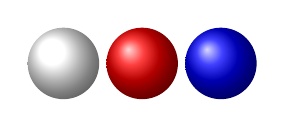
\begin{tikzpicture}
\shade[ball color=white] (0,0) circle (3ex) ;
\shade[ball color=red ] (1,0) circle (3ex) ;
\shade[ball color=blue ] (2,0) circle (3ex) ;
\end{tikzpicture}

\begin{tkzexample}[overhang,width=6cm,code=red!30]
\begin{tikzpicture}[scale=.4]
\tkzDefPoints{0/0/P,5/0/Q,3/2/I}
\tkzDefCircle[orthogonal from=P](Q,I)
\tkzGetFirstPoint{E}
\tkzDrawCircles(P,E Q,E)
\tkzInterCC[common=E](P,E)(Q,E) \tkzGetFirstPoint{F}
\tkzDefPointOnCircle[through = center P angle 80 point E]
\tkzGetPoint{A}
\tkzInterLC[common=E](A,E)(Q,E) \tkzGetFirstPoint{C}
\tkzInterLL(A,F)(C,Q) \tkzGetPoint{D}
\tkzDrawLines[add=0 and .75](P,Q)
\tkzDrawLines[add=0 and 2](A,E)
\tkzDrawSegments(P,E E,F F,C A,F C,D)
\tkzDrawPoints(P,Q,E,F,A,C,D)
\tkzLabelPoints(P,Q,F,C,D)
\tkzLabelPoints[above](E,A)
\end{tikzpicture}
\end{tkzexample}


\section{数式を書いてみる}
\[ \left( \int_0^\infty \frac{\sin x}{\sqrt{x}} dx \right)^2=
\sum_{k=0}^\infty \frac{(2k)!}{2^{2k}(k!)^2} \frac{1}{2k+1}=
\prod_{k=1}^\infty \frac{4k^2}{4k^2 -1}= \frac{\pi}{2} \]

\section{表を作成する}
\centering{%
\begin{tabular}{lrr}
\hline 品名 & 単価(円) & 個数
\\ \hline りんご & 100 & 5
\\ みかん & 50 & 10
\\ マンゴ & 300 & 8
\\ \hline
\end{tabular}}

\section{画像を取り込む}
\centering{%
\includegraphics[width=3cm,clip] {tiger.png}}


%\ifSubfilesClassLoaded{
%\bibliographystyle{unsrt}
%\bibliography{ref2.bib}
%}{}


\end{document}
%% ---------------------------------------------------------------------
%% coding: utf-8
%% version-control: t
%% kept-new-versions: 3
%% kept-old-versions: 0
%% End:
%% sub1.tex ends here
